\documentclass[a4paper,10pt]{article}
\usepackage[utf8x]{inputenc}
\usepackage{graphicx}
\usepackage{amsmath}

%opening
\title{Assignement 2}
\author{Shuying Dong, Roman Karlstetter}

\begin{document}



\section{Das Gesetz von Amdahl}
\renewcommand{\labelenumi}{\alph{enumi})}
\begin{enumerate}
 \item 
\begin{align*}
Eff &= \frac{Sp}{p} \geq 70 \% \\
Eff &\leq  \frac{Sp}{p} = \frac{\frac{1}{s+{\frac{1-s}{p}}}}{p} = \frac{1}{(s+{\frac{1-s}{p}}) \cdot p}  = \frac{1}{s\cdot p+1-s}\\
\frac{1}{Eff} &\geq  s\cdot p+1-s\\
\frac{1}{Eff} -1 + s &\geq  s\cdot p\\
\frac{\frac{1}{Eff} -1 + s}{s} &\geq  p\\
\frac{\frac{1}{0.7} -1 + 0.1}{0.1} = 5.286 &\geq  p\\
\end{align*}

You can therefore use at most 5 processes to have a parallel efficiency of 70\%, when the serial part of your code is 10\%.
\item 
Choose some fixed s. Then we can say: 
\begin{align*}
 \lim\limits_{p \rightarrow \infty}{Sp} &= \lim\limits_{p \rightarrow \infty}{\frac{1}{s+{\frac{1-s}{p}}}}\\
&= \lim\limits_{p \rightarrow \infty}{\frac{1}{s}} = \frac{1}{s}\\
\end{align*}

The meaning of this equation is that the speedup you can achieve is the inverse of the serial fraction of your programm, so for example, if 20 \% of your programm are sequential (i.e. can not be serialized), then the theoritical maximum speedup you can get is 5 (with an infinite amount of processes).

Amdahl's law always looks at a fixed problem size and therefore, also the sequential part of the programm requires always the same share of computations. When we allow the problem size to change, we can possibly increase the amount of data which can be procesed in parallel, and therefore the fraction of the serial code can me reduced, as sequential parts of the programm often are things which have to be performed only once (stuff like initialization etc.). 

Gustafsons law formalizes this idea. It states that "problems with large, repetitive data sets can be efficiently parallelized" (wikipedia). As a consequence, an algorithm which does more computations on many parallel machines might be (in total) faster than an algorithm with a minimized amount of computations but no parallelism.
\end{enumerate}

\section{Broadcast}
\begin{itemize}
 \item process 0 sends the complete array to every other process. This means that it has to send $n \cdot (p-1) \cdot sizeof(double) = n \cdot (p-1) \cdot 8$ Bytes and $p-1$ MPI-messages in total. As we send only from one process, this is the critical path. (The total amount of sent data does not differ in the other cases)
 \item Here, the critical path is as illustrated in the image: This means that there are $\lceil log_2(p) \rceil + 1$ levels in the tree. Therefore, there have to be sent  $\lceil log_2(p) \rceil$ packages on this path, each containing $n \cdot 8$ Bytes.
\begin{figure}[h!]
 \centering
 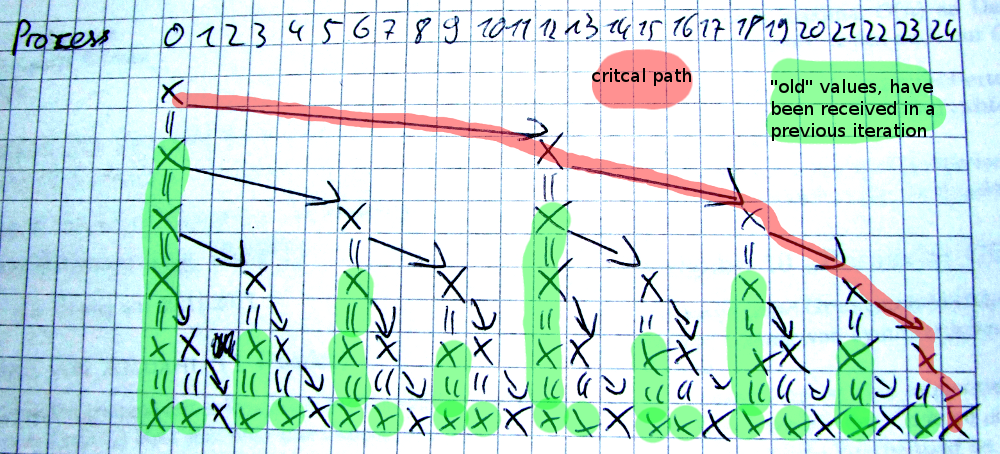
\includegraphics[width=0.9 \textwidth]{09/tree_critical_path.png}
\end{figure}

 \item In this case, we split up our array in p-1 parts. In the first iteration process 0 sends the first part of the array to process 1, the second part of the array to process 2 and so on. Then, the processes send the parts of the array is in the picture, which means, that in this case, a/every process sends $(p-1)$ Packages of size $\frac{n}{p-1}$, so in total $(p-1) \cdot \frac{n}{p-1} \approx n \in \varTheta(n)$. As every process send approximately the same amount of data, on the critical path there is not more data sent. 

There are probably more clever implementations for small n (especially up to p).
\begin{figure}[h!]
 \centering
 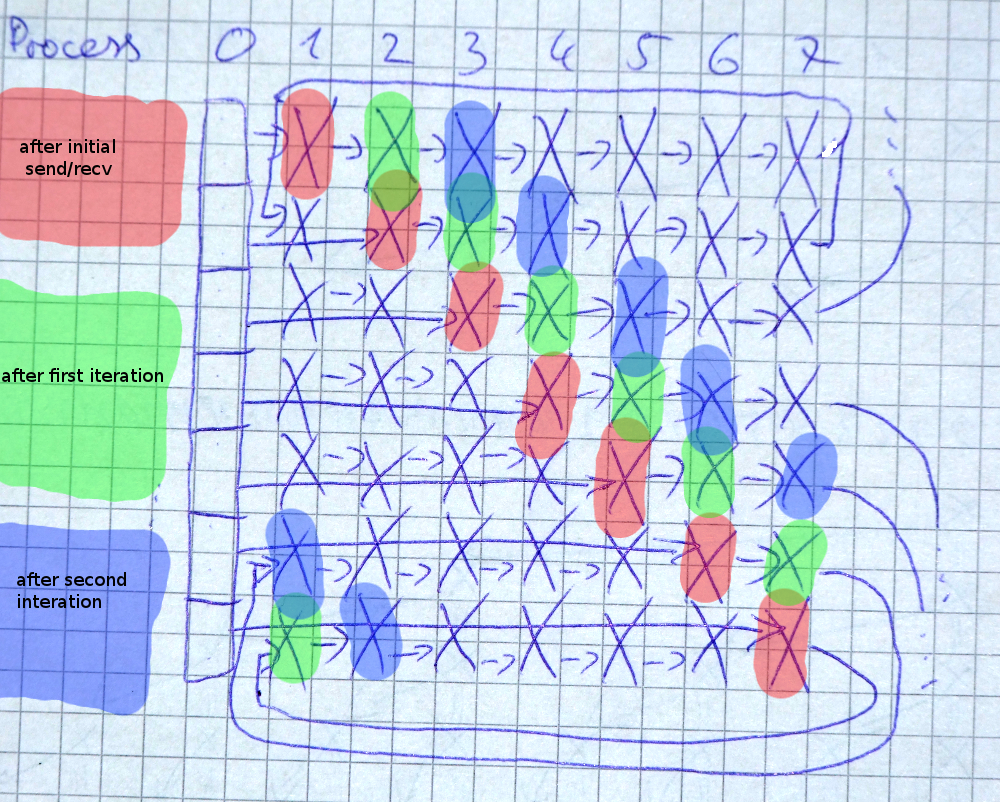
\includegraphics[width=0.8 \textwidth]{09/bonus_critical_path.png}
\caption{bonus critical path}
\end{figure}
\end{itemize}

This is the analysis of the bandwidth:

\begin{figure}[h!]
 \centering
 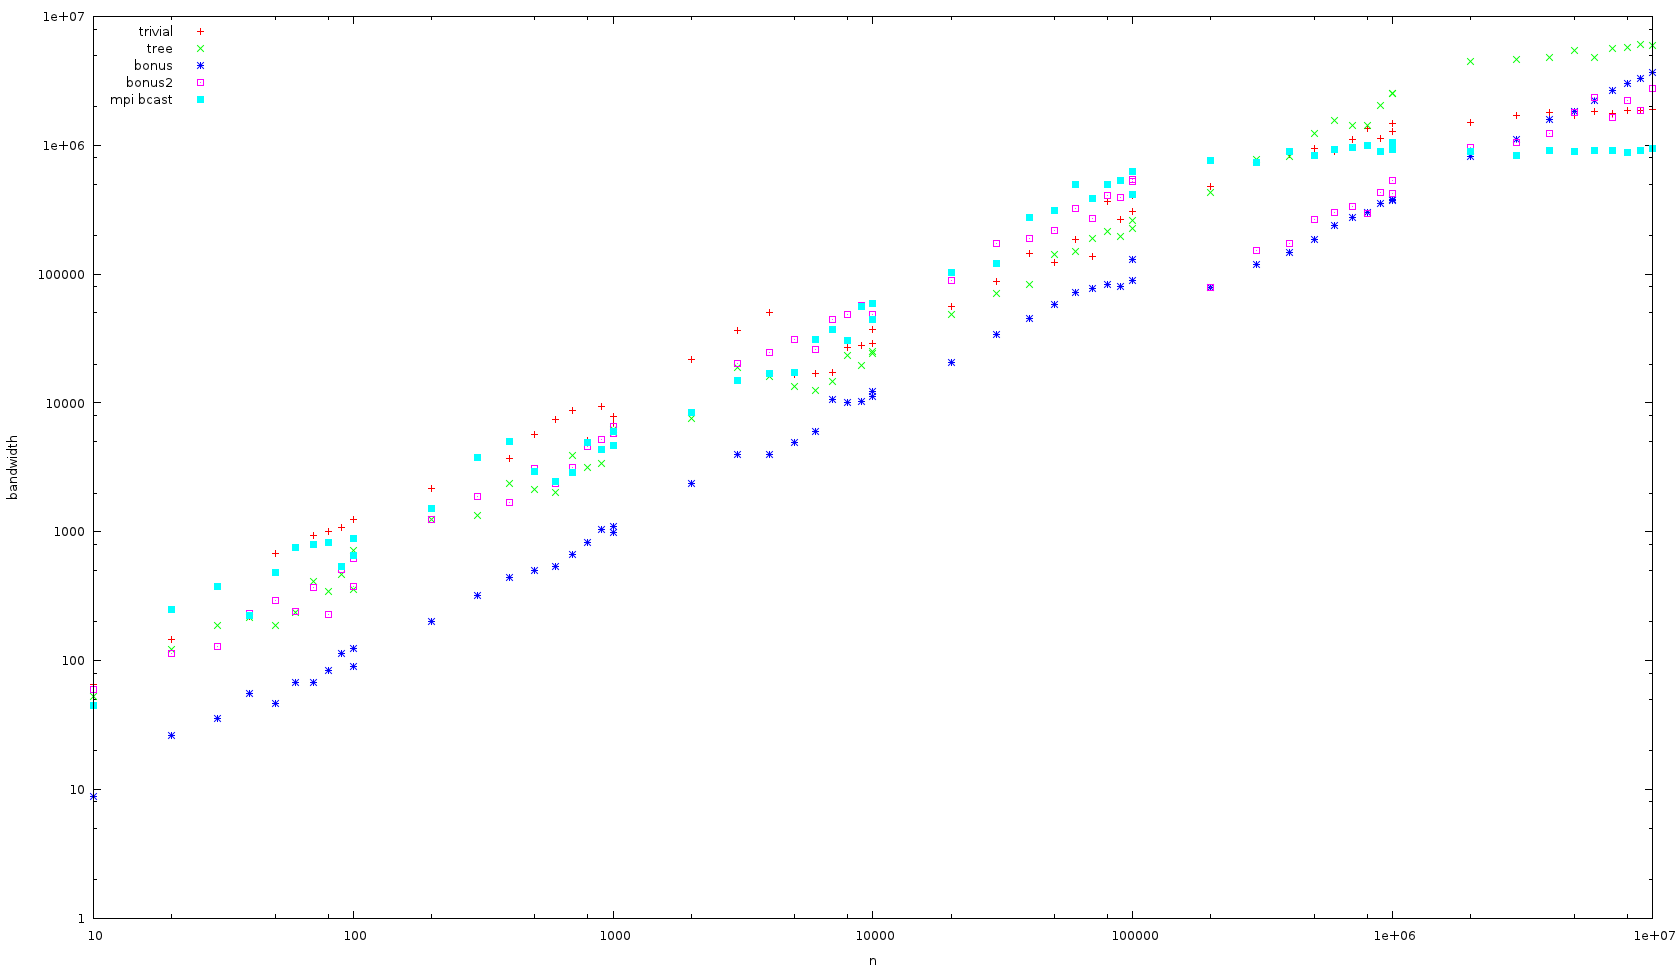
\includegraphics[width=1.1 \textwidth]{09/bandwidth.png}
\end{figure}

\section{Paralleles CG}

\end{document}
